\chapter{Onderzoek: Architectuur binnen Eaglescience}\label{ch:onderzoek:-architectuur-binnen-eaglescience}

Dit hoofdstuk beschrijft het onderzoek naar de manier waarop EagleScience software ontwikkeld en uitrold. Als eerst wordt de onderzoeksvraag ontleed in te beantwoorden deelvragen. Daarna zal er wordt iedere deelvraag beantwoord om vervolgens tot een conclusie te komen welke de onderzoeksvraag beantwoord en als input dient voor het laatste onderzoek over een methode voor een \textit{SOUP} analyse

%wellicht nog handig als er toch een reden  moet zijn waarom ES Scala gebruikt
%https://www.lihaoyi.com/post/FromFirstPrinciplesWhyScala.html#conclusion-all-languages-lead-to-scala
\section{Onderzoeksvragen}\label{sec:ESOnderzoeksVraag}
De onderzoeksvraag die als startpunt van dit onderzoek geld is: "Welke methode en dev-stack worden er binnen EagleScience gebruikt om software te ontwikkelen en uit te rollen?". Om deze vraag volledig te kunnen beantwoorden is deze in de volgende deelvragen opgedeeld:
\begin{itemize}
    \item Welk proces wordt er binnen Eaglescience gebruikt om software te ontwikkelen en hoe resulteert dit is een dagelijkse werkwijze?
    \item Wat zijn de meest gebruikte ontwikkeltalen en frameworks die binnen EagleScience worden toegepast?
    \item Welke tooling wordt er gebruikt binnen EagleScience? [NOTE relevant?]
    \item Hoe wordt er binnen EagleScience software uitgerold?
\end{itemize}


\section{Dagelijkse werkwijze}\label{sec:dagelijkse-werkwijze}
Om antwoord te krijgen op de vraag: "Welk proces wordt er binnen Eaglescience gebruikt om software te ontwikkelen?" Moet er gekeken worden hoe EagleScience werkt op dagelijkse basis.

Binnen Eaglescience wordt er getracht om "full Scrum" te werken. Dit wil zeggen dat voor ieder project een team van maximaal 9 full-stack developers wordt aangewezen. De sprints duren ongeveer 2 á 3 weken afhankelijk van wensen van de klant en beschikbaarheid van ontwikkelaars. Iedere sprint begint met een refinement waarbij de taken die op de backlog staan worden bekeken en ingeschat door het team. Tijdens de sprint vindt de ontwikkeling middels taken plaats die vervolgens worden gereviewd door een ander teamlid. Aan het einde van de sprint vind er een retrospective plaats en eventueel een demo om de voortgang te demonstreren aan de klant, dit is ook het moment dat het team ziet hoe de applicatie in het algemeen werkt. Dit is ook het moment voor de projectmanager en product owner om de taken die op de back-log staan opnieuw te prioriseren waarbij in de refinement van de volgende sprint de taken mee wordenblue genomen.

[NOTE: Wellicht onder tooling te plaatsen.]
Om deze werkwijze te ondersteunen maakt EagleScience gebruik van de een PO(T)AP(Personal, Development, (Test)/Acceptence, Production) omgevingen die middels Jenkins worden gebuild naar de desbetreffende omgeving. Alle genoemde omgevingen worden gemonitord middiels azure portal echter draaien de peronal en developement omgevingen lokaal op een server. Alle omgevingen behalve personal draaien middels docker containers in een kubernetes services. Iedere ontwikkelaar heeft zijn eigen omgeving die hij kan bouwen om te testen of aanpassingen werken zoals verwacht welke in docker containers draaien lokaal op een server. Er is per project een Ontwikkelomgeving waarin getest wordt of alle aanpassingen van de ontwikkelaars met elkaar werken. De acceptatieomgeving is er voor de projectmanagers en testers vanuit de klant of desgewenst externe testers om de ontwikkelde applicatie te testen zoals hij naar productie zou gaan. De productie omgeving host alle applicaties die 'live' zijn. Gezien alle omgevingen in docker containers draaien zijn deze volitile en kunnen dus "makkelijk" worden vervangen. zeker voor de personal en development omgeving wordt dit gezien als een voordeel vanwege het vele bouwen van deze omgevingen.

\begin{figure}[bth]
    \myfloatalign
    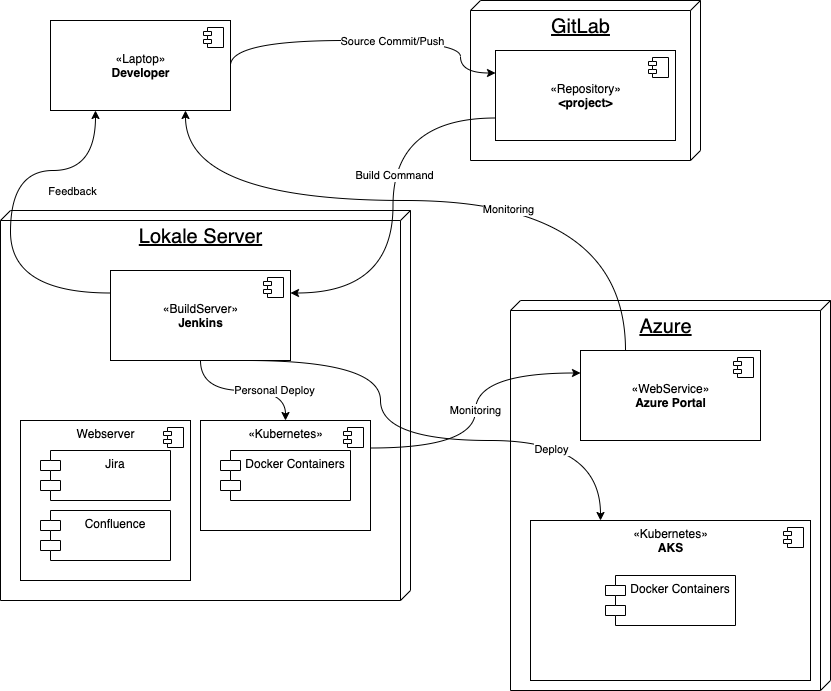
\includegraphics[width=10cm]{gfx/ES-BuildArchitecture}
    \caption{EagleScience Tooling}
    \label{fig:es-tooling}
\end{figure}



\section{Ontwikkeltalen en tooling binnen EagleScience}\label{sec:ontwikkeltalen-en-tooling-binnen-eaglescience}
EagleScience maakt volledige full stack oplossingen. Er wordt dus zowel front-end, backend, en database oplossingen ontwikkelt binnen projecten. Om deze reden wordt er binnen EagleScience gebruik gemaakt van verchillende ontwikkeltalen en tooling om projecten te voltooien. Hieronder staan de belangrijkste vermeld. Deze lijst is bij lange na niet volledig.

\subsection{OntwikkelTalen en frameworks}\label{subsec:ontwikkeltalen-en-frameworks}
Zoals eerder beschreven ontwikkelend EagleScience software full-stack. Er wordt dus gebruik gemaak van zowel talen voor de frontend en backend. Databases worden niet meegenomen in de lijst omdat deze als complete componenten worden gezien en de analyse op SOUP in deze ook niet veel zin heeft.
\begin{itemize}
    \item \textbf{Scala 2.XX} De voornamelijkst taal voor het ontwikkelen van de backend binnen EagleScience is Scala. De keuze voor deze taal is de mogelijkheid om functioneel te kunnen programmeren in de Java Virtual Machine(JVM) draait. Dat laatste zorgt ervoor dat bibliotheken die geschreven zijn in talen die ook ondersteunt worden door de JVM gebruikt kunnen worden ongeacht of deze in Scala, Java, Groovy of Kotlin geschreven zijn. Naast dit feit is Scala uiterst geschikt om software te bouwen dat schaalbaar is. Scala heeft de mogelijkheid om mee te groeien met het project. En heeft dus de mogelijkheid om zowel in gezet te worden als script taal dan al niet in Java applicaties als ook de mogelijkheid om production ready applicaties te bouwen die mee schalen in het gebruik. De naam Scala is dan ook een samenraapsel van de woorden scalable en language.
    EagleScience maakt gebruik van deze taal omdat Scala de mogelijkheid geeft om een applicatie makkelijk uit te breiden als dit nodig is. De ondersteuning voor functioneel programeren geeft het voordeel dat de geschreven code makkelijker te testen valt. (pure)functies hebben de eigenschap deterministisch te zijn wat wil zeggen dat iedere keer als een bepaalde input in een functie komt er altijd dezelfde output verwacht kan worden. Deze eigenschap maakt het mogelijk om applicaties sneller en makkelijker te testen. Binnen EagleScience worden er in bijna alle projecten een aantal frameworks/bibliotheken gebruikt die het ontwikkelen van microservice web applicaties in Scala makkelijker maakt:
    \begin{itemize}
        \item \textbf{PlayFramework 2.xx} Een web framework voor de ontwikkeling van webapplicaties in Scala we gebruikten het vooral als router voor de verschillende microservices die er achterliggen.
        \item \textbf{ArchES} is een intern ontwikkeld framework wat de opbouw en de communicatie tussen microservices in scala verbeterd.\ ArchES is geinspireerd op Apache KAFKA en werkt middels hetzelfde pub -> sub principe.
    \end{itemize}
\end{itemize}

\subsection{Tooling}
Naast ontwikkeltalen gebruikt EagleScience een aantal tools om dagelijkse werkzaamheden te stroomlijnen en software uit te rollen voor de klant. De tools zijn ieder op zijn beurt verantwoordelijk voor een specifieke taak en alle projecten dienen gebruik te maken van deze tools waar gepast. Hoe de tools samenwerken en uitgerold zijn is te zien in figuur~\ref{fig:es-tooling}

\begin{itemize}
    \item \textbf{Jira} Is naar eigen zeggen (JiraWebsite ) de nummer 1 software ontwikkel tool voor agile teams.\ Eaglescience gebruikt het om projecten te plannen volgens de scrum methode.\ De tool maakt het mogelijk om sprints te plannen. Daarnaast maakt EagleScience gebruik van Jira om workflows te beheren. zoals interne zaken als toegangverlenen. Maar ook vastlegging van meldingen van klanten welke vervolgens door de ontwikkelaars worden opgepakt en onderzocht.
    \item \textbf{Confluence}
    Confluence wordt binnen Eaglsescience gebruikt als samenwerkings tool waarbij de documentatie centraal ligt.\ De omgeving bied de mogelijk om samen te werken met Jira waardoor documentatie makkelijk te vinden op zowel project als taak niveau.
    \item \textbf{GitLab}
    De Code Repository die Eaglescience gebruikt.
    \item \textbf{Jenkins}
    Jenkins is een open-source automation server wat door Eaglescience gebruikt wordt om projecten te builden voor verschillende doeleinden.\ Doordat Jenkins Open-source is zijn er veel plugins geschreven die de functionaliteit uitbreiden en het dus bruikbaar maakt voor het bouwen van een pipeline voor veel verschillende talen en frameworks.
    Jenkins kan worden vergeleken als mission control tijdens de lancering van een raket\ Voordat de raket(de deploy) gelanceerd kan worden, wordt er een go-nogo sequence uitgevoerd waarbij iedere stap een test of check is waar alleen een go of no-go uit kan komen.\ Op het moment dat alles op go staat is de build geslaagd en kan er gedeployed worden.\ Wil niet zeggen dat de deploy altijd geslaagd is met Jenkins.\ Er zijn nog een aantal andere factoren die meehelpen aan een geslaagde deploy zoals bijvoorbeeld bugs die niet uit de tests zijn gekomen.
\end{itemize}


\section{Hoe wordt op dit moment software gedeployed?}\label{sec:hoe-wordt-op-dit-moment-software-gedeployed?}
Zoals hierboven berschreven wordt Jenkins gebruikt om software te deployen naar zowel de productie omgevingen alsook de verschillende development en acceptatie omgevingen.
Een deploy wordt gedaan op het moment dat er source code naar gitlab gepushed wordt.
Doormiddel van Tokens in de Commit message kan gestuurd worden waar de build(als deze slaagt) gedeployed wordt bijv: {-all + portal} build en deployed alleen de portal. [ci-skip] zorgt ervoor dat er alleen een push wordt gedaan en geen build wordt gestart.
De configuratie die Jenkins gebruikt wordt beschreven in een aantal Jenkins files die meegenomen worden de repo. Middels parameters meegegeven in de commit kan er worden beslist of er een build moet plaatsvinden en zo ja waar en welke delen van de applicatie. Op deze manier is er een flexibiliteit voor de ontwikkelaar.
[NOTE Illustratie maken.....]
Naast de deploy geeft Jenkins nog een aantal andere waardevolle Artifacts als test/lint rapportages.
Een build en deploy gaat volgens de onderstaande afbeelding:

\begin{figure}[H]
    \myfloatalign
    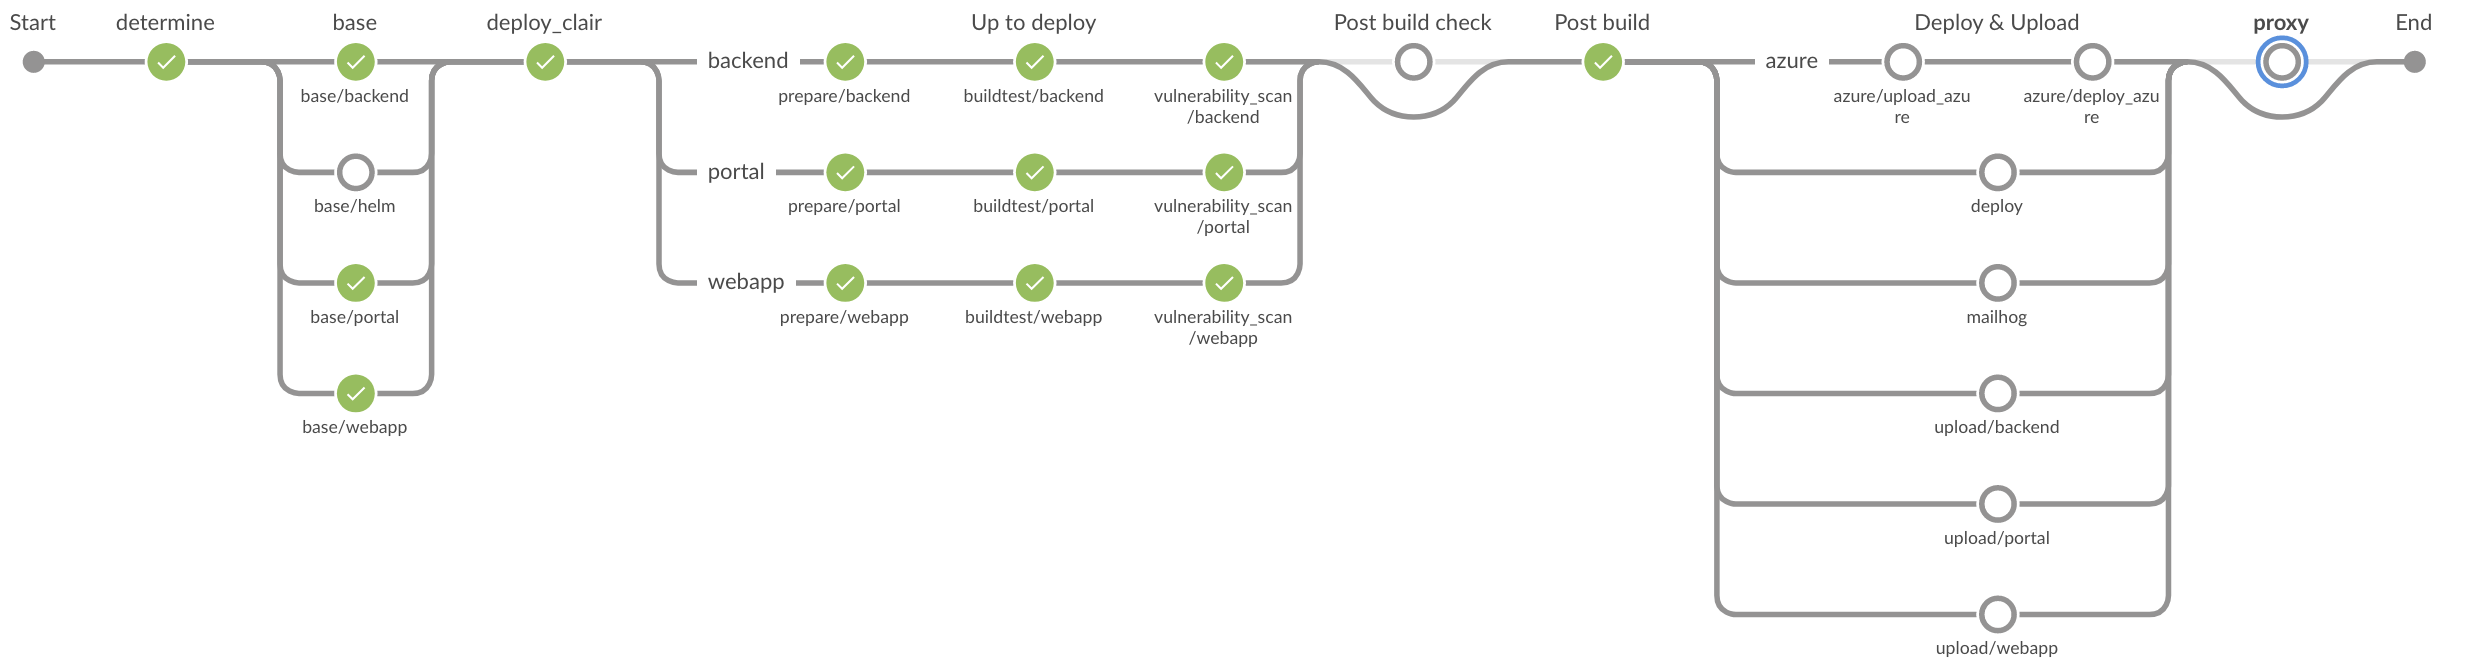
\includegraphics[width=15cm]{gfx/Screenshot 2021-08-18 Jenkins PipeLine}
    \caption{Jenkins(Blue Ocean) pipeline}
    \label{fig:JenkinsPipeLine}
\end{figure}
Een Jenkins pipeline werkt in een aantal stappen dat in een .jenkinsFile wordt beschreven.
Deze jenkinsFile wordt in de determine stap ingelezen en de benodigde stappen op een rij gezet.
De stappen die worden uitgevoerd zijn:
\begin{itemize}
    \item \textbf{determine} Nu wordt bekeken welke stappen er nodig zijn om een succesvolle build en of deploy te kunnen doen./ Aan de hand van een JenkinsFile en tokens in een Commit message wordt hier bekeken welke stappen er moeten worden uitgevoerd om tot een goed einde te komen.
    \item \textbf{base} In de base stap worden alle Containers voorbereid die nodig zijn om de applicatie te draaien.\ Images worden opgehaald en gedeployed De base stap is een parallel lopende stap waarin in dit geval backend, portal en de app worden voorbereid.
    \item \textbf{deploy clair} de clair scanner zoekt op kwetsbaarheden binnen containers die zojuist zijn aangemaakt.\ Dit is een extra veiligheid die ervoor zorgt dat de images en container veilig zijn er alleen nog door bibliotheken die gebruikt worden voor ontwikkeling kwetsbaarheden kunnen worden toegevoegd
    \item \textbf{Up to deploy}
    in dit geval wordt er voor de backend, portal, en app een parallel process gestart waarin alle drie substappen doorlopen:
    \begin{itemize}
        \item \textbf{prepare} Docker containers worden ingesteld, en klaar gezet voor het ontvangen van de services.
        \item \textbf{builtest} De services worden gebuild en gestest in deze stap.\ Eaglescience heeft een aantal tresholds opgesteld waaraan tests moeten voldoen om deze te analyseren worden de test resultaten vanuit de docker containers gekopieerd naar de Jenkins Store waar Jenkins de waarden kan analyseren als alle tests binnen de resultaten vallen wordt de volgende stap uitgevoerd.
        \item \textbf{vulnerability scan} Clair scanner scant nu de containers nogmaals maar nu op de gebruikte software.\ Als clair iets vind dat eaglescience als verdacht acht dan wordt de build gestaakt.
    \end{itemize}
    \item \textbf{PostBuild(check)}
    Alle bevindingen worden hier gecheckt mocht er iets mis zijn wordt er wederom afgebroken en is de build gefaald en kan er dus niet een deploy plaatsvinden.
    \item \textbf{Deploy \& Upload}
    in dit geval wordt de deploy niet uitgevoerd.\ Deze stap zorgt ervoor dat de gebouwde containers worden overgedragen naar Azure.\ Iedere container heeft wederom zijn eigen stappen.
    \item \textbf{End}
    Einde van de PipeLine Jenkins geeft de workers die het project heeft gebruikt weer vrij.
\end{itemize}


\section{Conclussie}
Binnen EagleScience wordt er gewerkt middels de SCRUM methode om software te ontwikkelen. Er vind dus op gezette tijden een uitrol plaats welke door Jenkins wordt uitgevoerd. De applicaties die uitgerold worden, zijn ontwikkeld in Scala en TypeScript met gebruik van zowel externe als interne bibliotheken om ontwikkeling te vergemakkelijken. Het lijkt dan ook voor de hand liggend om binnen Jenkins een mogelijkheid te hebben om gegevens over een build naar de nieuwe SOUP module over te brengen. Er zal daarnaast dus gezocht moeten worden naar een analyse tool die het mogelijk maakt om binnen NPM(package manager voor Node projecten) en SBT(Scala Build Tool) gegevens te generenen die in een module geplaatst kunnen worden.
